% !TeX root = 70-experiment.tex
\documentclass[dp.tex]{subfiles}
\begin{document}
\chapter{Praktická část}
\label{chap:experiment} 

Cílem diplomové práce je porovnání sledovaných charakteristik na různých českých překladech básně Havran. České překlady byly vydány nakladatelstvím Odeon v knize \citetitle{Poe1990}. Pro realizaci praktické části této diplomové práce budou použity překlady uvedené v knize, a to včetně dvou překladů (Vrchlického překlad vydaný roku 1881 v časopisu Lumír a čtvrté vydání překladu Kamilla Reslera vydaném Josefem Ciprou roku 1956) uvedených v komentáři Rudolfa Havla.

\section{Porovnání četností znaků}

Prvním porovnáním, které bylo v rámci praktické části realizováno, je srovnání četnosti znaků. Jak uvádí Jan Králík v \cite[str.~109]{Tesitelova1987}: 

\begin{quote}
Znalost míry užívání (frekvence) písmen stála u zrodu těsnopisných a telegrafních značek a dodnes tak úzce souvisí s ekonomikou záznamu a přenosu textových informací. Znalost frekvence písmen výrazně zasáhla i do uspořádání klávesnic u prvních psacích strojů sériově vyráběných; dodnes jsou proto psací stroje s latinkou vhodnější pro angličtinu, pro niž byly původně konstruovány, než pro kterýkoli jiný jazyk. Znalost frekvencí písmen se osvědčila i ve vojenství při dešifrování kódovaných zpráv: stačilo znát frekvence písmen v daném jazyce a porovnat je s frekvencemi užitých \clq tajných znaků\crq.
\end{quote}

Porovnáváno bylo všech osmnáct českých překladů, přičemž analýza byla nastavena tak, aby byla započítána pouze písmena, aby byla ignorována rozdílná velikost písmen a aby \glslink{bigram}{bigram} \clq ch\crq byl považován za jedno písmeno.

V takto nastavené analýze četnosti znaků bylo v testovaných textech nalezeno $69 368$ znaků, z toho však pouze $40$ znaků bylo unikátních (z české abecedy nebyly zastoupeny znaky \textit{Q} a \textit{W}). Nejčastěji se vyskytujícím znakem byl znak \textit{E}, který se vyskytl celkem $5530\times$. Následovaly znaky \textit{N}, \textit{A}, \textit{O}, a \textit{S}.

Námi nalezené četnosti porovnáme s četnostmi uvedenými na stránkách czech-language.cz\footnote{Dostupné on-line z \url{http://www.czech-language.cz/alphabet/alph-prehled.html}}. Tato frekvenční tabulka byla vytvořena na základě analýzy $3 139 926$ znaků. Na Internetu i v literatuře je možné najít i další frekvenční tabulky pro češtinu\footnote{on-line např. \url{https://nlp.fi.muni.cz/web3/cs/FrekvenceSlovLemmat}, \url{http://www.sttmedia.com/characterfrequency-czech}, \url{http://www.cryptogram.org/cdb/words/frequency.html}, v literatuře např. \citetitle{Kraus1965} (viz \cite{Kraus1965}), částečně \citetitle{Tesitelova1987} \cite[str.~109-121]{Tesitelova1987}.}.

\begin{figure}[h!]
	\centering
	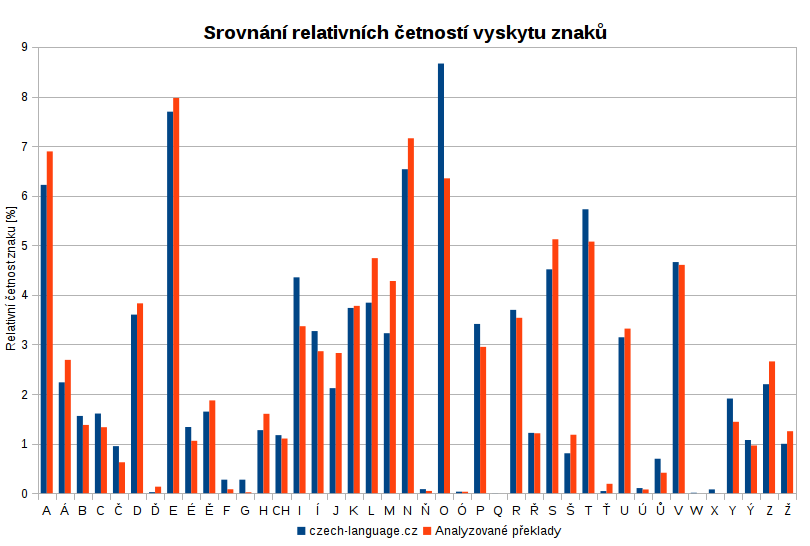
\includegraphics[max width=\textwidth,keepaspectratio=true]{imgs-70-prakticka/cetnost-znaku2}
	\caption[Srovnání relativních četností výskytu znaků v analyzovaných překladech.]{Srovnání relativních četností výskytu znaků v analyzovaných překladech. \textit{Zdroj:~vlastní.}}
	\label{fig:character-freq}
\end{figure}

Graf \ref{fig:character-freq} zachycuje poměr mezi relativními četnostmi výskytu jednotlivých znaků v analyzovaných překladech. V grafu vidíme, že naměřené hodnoty korespondují s hodnotami z referenční frekvenční tabulky. Nejvyšší odchylka se vyskytla u znaku \textit{O}, činí $2,32 \%$.

\section{Porovnání četností slov}

Zkoumání počtu výskytů jednotlivých slov v daném jazyce je typickou úlohou kvantitativní lingvistiky. Její výsledky mohou být použity při konstruování slovníků a jazykových učebnic, k identifikaci klíčových slov v textech, k poměřování mezi alternujícími slovy (např. \enquote{bychom} a \enquote{bysme}), k nalezení ustálených slovních spojení aj.\footnote{Zdroj: \url{https://wiki.korpus.cz/doku.php/pojmy:frekvence\#vyuziti_a_vyznam_frekvence}.}.

To, kolikrát se které slovo vyskytuje, uvádějí tzv. frekvenční slovníky nebo seznamy. Pro češtinu existuje několik takových slovníků (\cite[str.~18]{Tesitelova1987}), např. \cite{Jelinek1961}, \cite{Tesitelova1980}, \url{https://ucnk.ff.cuni.cz/srovnani10.php}. Výsledky analýzy četnosti znaků budou porovnány s následujícími frekvenčními seznamy:
\begin {table}[H]
	\caption {Srovnání frekvenčních slovníků} \label{tab:title} 

	\begin{center}
		\begin{tabular}{{l|l|l|l}}
		\hline
		\bfseries \bfseries Název & \bfseries Rok publikace & \bfseries Zdroj & \bfseries Velikost zdrojového souboru [slova]\\
		    \hline \hline
		   Jelínek 1961    & 1961 & \cite{Jelinek1961}    &    1 623 527   \\\hline
		   Těšitelová 1983 & 1983 & \cite{Tesitelova1980} &     540 000    \\\hline
		   Čermák 2004     & 2004 & \cite{Cermak2004}     & 100 000 000    \\\hline
		\end{tabular}
	\end{center}
	\label{tab:word-freq-lists}
\end{table}

V rámci ukázky analýzy četnosti slov budou předvedena dvě porovnání:
\begin{enumerate}
\item V českých překladech bude sledován počet slov se zaměřením na slova odkazující na \enquote{havrana} (tj. slova \enquote{havran} a \enquote{pták} + jejich tvary).
\item České překlady budou porovnány s anglickým originálem. Porovnáván bude počet odkazů na havrana v originálu (anglická slova \enquote{raven} a \enquote{bird}) s českým \enquote{havran} a \enquote{pták} v jednotlivých překladech.
\end{enumerate}

\subsection{Analýza českých překladů}
\label{chap:word-freq-list} 

Analýza četnosti slov byla nastavena tak, aby byla slova porovnávána dle obsahu a aby byla ignorována velikost písmen. Vzhledem k tomu, že vyvinutý program nepodporuje žádný slovník tvarů slov, bylo nutné přidat do analýzy taková pravidla, aby byly i výskyty různých tvarů slov \enquote{havran} a \enquote{pták} připočteny k výskytům \glslink{lemma}{lemmat}. Pro slovo \enquote{havran} se jednalo o tvary \textit{havrana}, \textit{havrane}, \textit{havráně} a \textit{havrany}. Tvary slova \enquote{pták}, které se nachází v jednotlivých překladech, jsou: \textit{ptáka}, \textit{ptákem}, \textit{ptákovi}, \textit{ptáku} a \textit{ptáků}.

Osmnáct testovaných překladů obsahuje celkem $16 091$ slov, z nichž bylo $3938$ slov unikátních. Nejčastěji se vyskytujícím slovem bylo slovo \enquote{v} ($425$ výskytů) následované slovy \enquote{se} (nalezeno $349\times$) a \enquote{jsem} ($331$ výskytů). \enquote{Havran} se se $173$ výskyty umístil na $7.$ místě, \enquote{pták} na místě $9.$, když byl nalezen $149\times$.

Na obrázku \ref{fig:word-freq} je vyobrazeno porovnání relativních četností výskytu deseti nejčastějších slov v analyzovaných překladech s četnostmi pocházejícími z frekvenčních seznamů uvedených v tabulce \ref{tab:word-freq-lists}.

\begin{figure}[h!]
	\centering
	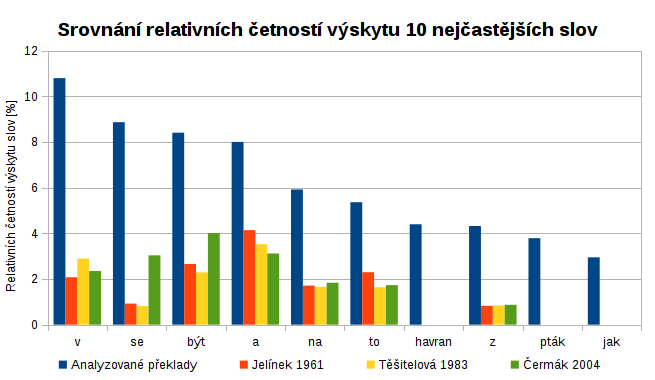
\includegraphics[max width=\textwidth,keepaspectratio=true]{imgs-70-prakticka/cetnost-slov}
	\caption[Srovnání relativních četností výskytu 10 nejčastějších slov v analyzovaných překladech.]{Srovnání relativních četností výskytu 10 nejčastějších slov v analyzovaných překladech. \textit{Zdroj:~vlastní.}}
	\label{fig:word-freq}
\end{figure}

V grafu vidíme, že relativní četnosti v analyzovaných překladech dosahují vyšších hodnot než ve frekvenčních seznamech. To je způsobeno jednak rozdílnou velikostí zkoumaného souboru textů a jednak vzájemnou podobností (a tím nižší variabilitou) českých překladů. 

Vůbec nejčastějším slovem v českých překladech byla předložka \enquote{v}. Ta se v referenčních seznamech umístila dvakrát na čtvrtém (Jelínek 1961), třetím (Čermák 2004) a druhém (Těšitelová 1983) místě. \enquote{V} se nejčastěji vyskytuje v překladu Jaroslava Vrchlického z roku 1881 ($36\times$). Poměrně často se také vyskytuje v Reslerově překladu ($30$ výskytů). Tyto překlady jsou v testovaném souboru zastoupeny dvěma vydáními, a přestože se jednotlivé verze odlišují, slovo \enquote{v} je v nich zastoupeno nadprůměrně.

Nadprůměrně je zastoupeno také slovo \enquote{jak}, kterému v Jelínkově seznamu patří 29. a v Čermákově dokonce až 36. místo. Nadprůměrně jsou zastoupeny také slova \enquote{havran} a \enquote{pták}, což pochopitelně souvisí s charakterem testovaného souboru. V tabulce \ref{tab:word-raven-bird-compare} je uvedeno pořadí výskytu slov \enquote{havran} a \enquote{pták} z \enquote{reprezentativnějších} seznamů\footnote{Ze seznamu Těšitelová 1983 má autor k dispozici pouze deset nejfrekventovanějších slov uvedených v \cite[str.~19]{Tesitelova1987}, proto není v tabulce uveden.}. 

\begin {table}[H]
	\caption {Srovnání pořadí výskytu slov \enquote{havran} a \enquote{pták}}
	\label{tab:srovnani-poradi-vyskytu-slov} 

	\begin{center}
		\begin{tabular}{{l||c|c}}
		\hline
		\bfseries  & \bfseries Pořadí v seznamu Jelínek 1961 & \bfseries Pořadí v seznamu Čermák 2004 \\
		    \hline \hline
		   \bfseries Havran    & 7895. &   5446.   \\\hline
		   \bfseries Pták& 991. &     2295.    \\\hline
		\end{tabular}
	\end{center}
	\label{tab:word-raven-bird-compare}
\end{table}

\subsection{Porovnání českých překladů s originálem}

Pro porovnání českých překladů s originálem budou parametry analýzy nastaveny stejně jako při porovnání s frekvenčními seznamy v kapitole \ref{chap:word-freq-list}. Navíc budou zavedena dvě nová pravidla zodpovědná za nahrazení anglického \enquote{raven} českým \enquote{havran} a anglického \enquote{bird} českým \enquote{pták}. Tím bude usnadněno porovnání jednotlivých překladů s originálním textem.

Na obrázku \ref{fig:word-freq-compare} je znázorněno srovnání četností výskytů slov \enquote{havran} (respektive \enquote{raven}) a pták (\enquote{bird}) v českých překladech a v originále. 

\begin{figure}[h!]
	\centering
	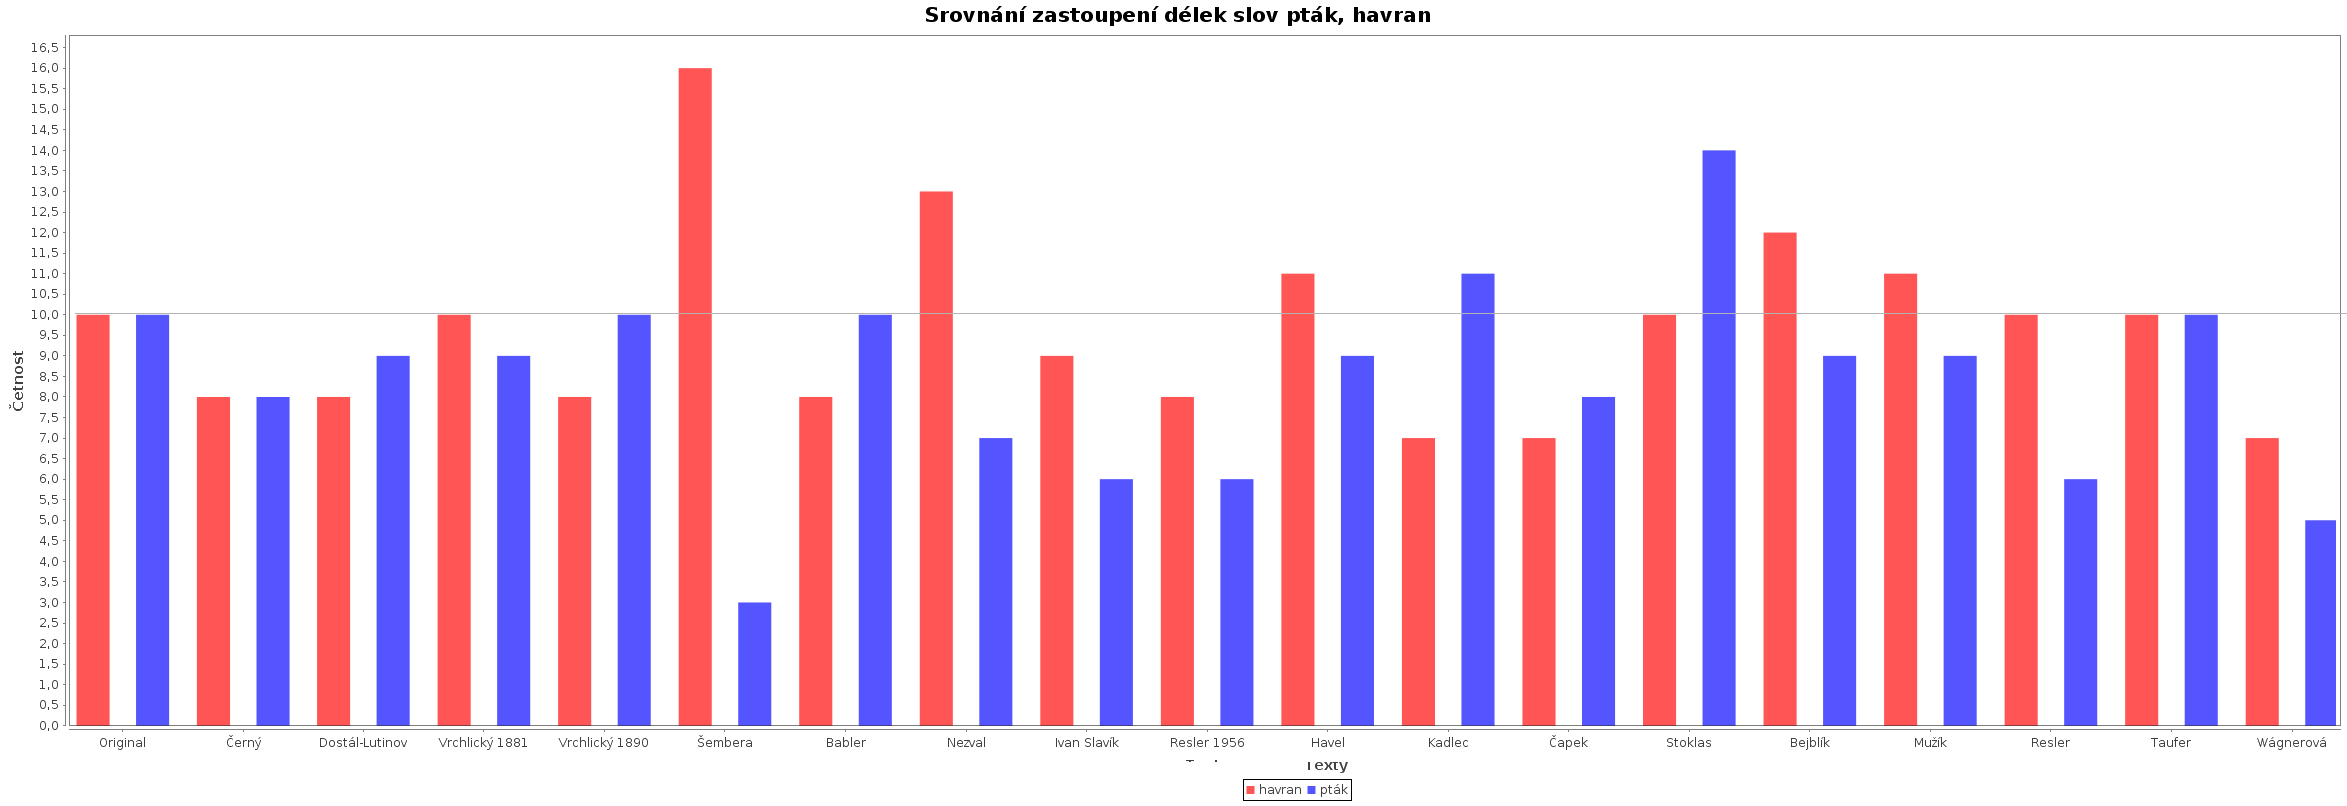
\includegraphics[max width=\textwidth,keepaspectratio=true]{imgs-70-prakticka/cetnost-slov-orig}
	\caption[Srovnání četností výskytů slov \enquote{havran} a \enquote{pták} v originále a v 18 českých překladech.]{Srovnání četností výskytů slov \enquote{havran} a \enquote{pták} v originále a v 18 českých překladech. \textit{Zdroj:~vlastní.}}
	\label{fig:word-freq-compare}
\end{figure}

V anglickém originálu se obě slova vyskytla desetkrát. Z českých překladů dosahuje stejných četností pouze překlad Jiřího Taufera. Ve Vrchlického překladu z roku 1881 najdeme \enquote{havrana} stejně jako v originále $10\times$, \enquote{pták} je však obsažen pouze devětkrát. Za povšimnutí stojí, že ve verzi vydané roku 1890 se \enquote{pták} vyskytuje již $10\times$, ovšem počet výskytů \enquote{havrana} klesl na osm. Od originálu o dva výskyty se lišící jsou i překlady Rudolfa Havla a Augustina Eugena Mužíka -- v obou se shodně nachází \enquote{havran} jedenáctkrát a \enquote{pták} devětkrát.

\section{Agregace}
\section{Asonance}
\section{Aliterace}
\section{Denotační analýza}
\label{chap:denotation-analysis} 

V rámci denotační analýzy byly etablovány hřeby pro poslední sloku všech osmnácti českých překladů. K omezení délky textů na pouze poslední sloku bylo přistoupeno zejména z důvodu složitosti takové analýzy. Jak uvádí Wimmer v \cite[str.~300]{Wimmer2003}: 

\begin{quote}
Treba poznamenať, že táto analýza je relatívne jednoduchá v krátkých textoch. Pri dlhých textoch bude pravdepodobne potrebné text najprv zakódovať, aby sa dal mechanicky spracovať, lebo pravdebodobnosť omylu stúpá od vety k vete.
\end{quote}

Na CD přiloženém k této diplomové práci jsou umístěny soubory obsahující jednak analyzované poslední sloky jednotlivých překladů a jednak samotné rozdělení těchto slok do hřebů. Jak bylo popsáno v kapitole \nameref{chap:app-denotation-analysis}, je možné tyto soubory použít k vlastní analýze. Elektronická příloha také obsahuje koincidenční a dererministicko-pravděpodobnostní grafy pro všechny překlady. Ty nejzajímavější jsou uvedeny přímo v této práci.

\subsection{Parametr $\alpha$}

Zásadní vliv na uspořádání výsledného grafu má zvolená hodnota hladiny významnosti $\alpha$. Výchozí hodnota hladiny významnosti je nastavena na $\alpha=0{,}1$, přičemž program umožňuje její hodnotu měnit v intervalu $\langle 0{,}001;1\rangle$ s krokem $0{,}001$.

Pokud je zvolená hodnota $\alpha$ příliš nízká, obsahuje výsledný graf mnoho izolovaných vrcholů. Čím je naopak hodnota $\alpha$ vyšší, tím je vyšší i počet hran grafu. Pro zvolení vhodné hodnoty je třeba experimentovat. 

Následující obrázky \ref{fig:denotation-resler-005}, \ref{fig:denotation-resler-007}, \ref{fig:denotation-resler-034}  zobrazují koincidenční grafy vytvořené na základě denotační analýzy poslední strofy Reslerova překladu. Pro všechna $\alpha \leq 0{,}5$ tvoří graf pouze izolované vrcholy ($0{,}5$ je tedy hodnota indexu nespojitosti). Při hodnotě $\alpha = 0{,}5$ dojde k vytvoření hrany mezi vrcholy $8$ a $9$. Při $\alpha = 0{,}7$ vznikne hrana i mezi vrcholy $6$ a $7$. K další redukci počtu komponent dojde při $\alpha = 0{,}17$, kdy dojde k propojení vrcholu $1$ s vrcholem $2$ a vrcholu $4$ s vrcholem $5$. Při $\alpha = 0{,}2$ se počet komponent sníží na $5$. V tu chvíli zbývají v grafu pouze dva izolované vrcholy -- $3$ a $10$. Při $\alpha = 0{,}34$ dojde k propojení vrcholu $3$ s komponentou tvořenou vrcholy $1$ a $2$. Poté v grafu zůstane jediný izolovaný vrchol -- $10$ -- k jehož propojení s jiným vrcholem nedojde, neboť index nespojitosti je roven $\infty$.

\begin{figure}[H]
	\centering
	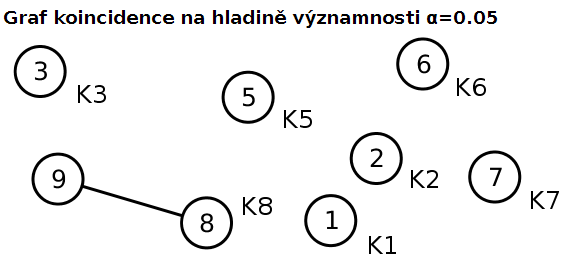
\includegraphics[max width=\textwidth,keepaspectratio=true]{imgs-70-prakticka/denotation-resler-005}
	\caption[Koincidenční graf Reslerova překladu pro $\alpha = 0{,}05$.]{Koincidenční graf Reslerova překladu pro $\alpha = 0{,}05$. \textit{Zdroj:~vlastní.}}
	\label{fig:denotation-resler-005}
\end{figure}

\begin{figure}[H]
	\centering
	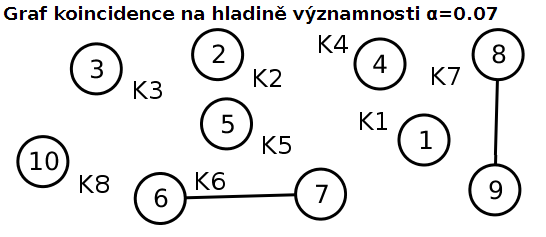
\includegraphics[max width=\textwidth,keepaspectratio=true]{imgs-70-prakticka/denotation-resler-007}
	\caption[Koincidenční graf Reslerova překladu pro $\alpha = 0{,}07$.]{Koincidenční graf Reslerova překladu pro $\alpha = 0{,}07$. \textit{Zdroj:~vlastní.}}
	\label{fig:denotation-resler-007}
\end{figure}

\begin{figure}[H]
	\centering
	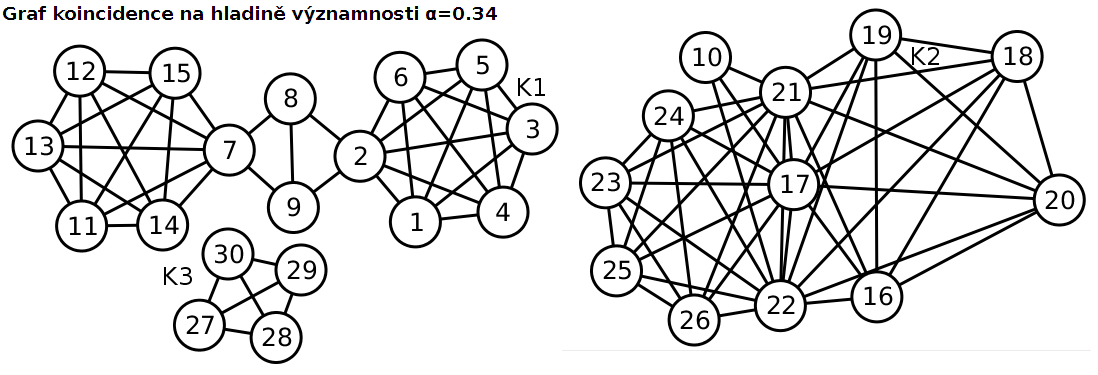
\includegraphics[max width=\textwidth,keepaspectratio=true]{imgs-70-prakticka/denotation-resler-034}
	\caption[Koincidenční graf Reslerova překladu pro $\alpha = 0{,}34$.]{Koincidenční graf Reslerova překladu pro $\alpha = 0{,}34$. \textit{Zdroj:~vlastní.}}
	\label{fig:denotation-resler-034}
\end{figure}

V tabulce \ref{tab:prehled-indexu-grafy} jsou uvedeny indexy nespojitosti, neizolovanosti a dosáhnutelnosti všech osmnácti analyzovaných překladů:

\begin {table}[H]
	\caption {Přehled indexy nespojitosti, neizolovanosti a dosáhnutelnosti} 
	\label{tab:prehled-indexu-grafy} 

	\begin{center}
		\begin{tabular}{{l|r|r|r}}
		\hline
		\bfseries \bfseries Překlad & \textbf{Index nespojitosti} & \bfseries Index neizolovanosti & \bfseries Index dosáhnutelnosti\\
		    \hline \hline
		   V. K. Šembera     & $0{,}067$ & $0{,}333$  &    $0{,}333$  \\\hline
		   J. Vrchlický 1881 & $0{,}067$ & $0{,}333$  &    $\infty$   \\\hline
		   J. Vrchlický 1890 & $0{,}055$ & $\infty$   &    $\infty$   \\\hline
		   A. E. Mužík       & $0{,}182$ & $\infty$   &    $\infty$   \\\hline
		   K. Dostál-Lutinov & $0{,}167$ & $\infty$   &    $\infty$   \\\hline
		   V. Nezval         & $0{,}167$ & $\infty$   &    $\infty$   \\\hline
		   O. F. Babler      & $0{,}167$ & $\infty$   &    $\infty$   \\\hline
		   J. Taufer         & $0{,}167$ & $\infty$   &    $\infty$   \\\hline
		   E. Stoklas        & $0{,}167$ & $\infty$   &    $\infty$   \\\hline
		   D. Wagnerová      & $0{,}055$ & $0{,}364$  &    $\infty$   \\\hline
		   R. Havel          & $0{,}167$ & $\infty$   &    $\infty$   \\\hline
		   J. B. Čapek       & $0{,}167$ & $\infty$   &    $\infty$   \\\hline
		   K. Resler 1948    & $0{,}050$ & $\infty$   &    $\infty$   \\\hline
		   K. Resler 1956    & $0{,}067$ & $\infty$   &    $\infty$   \\\hline
		   R. Černý          & $0{,}167$ & $\infty$   &    $\infty$   \\\hline
		   I. Slavík         & $0{,}167$ & $\infty$   &    $\infty$   \\\hline
		   S. Kadlec         & $0{,}067$ & $\infty$   &    $\infty$   \\\hline
		   A. Bejblík        & $0{,}067$ & $\infty$   &    $\infty$   \\\hline
		\end{tabular}
	\end{center}
	\label{tab:word-freq-lists}
\end{table}

\end{document}
